\documentclass[12pt,a4paper]{article}

\usepackage[utf8]{inputenc}
\usepackage{amsmath, amssymb, amsthm}
\usepackage{graphicx}
\usepackage{float}
\usepackage{booktabs}
\usepackage{siunitx}
\usepackage{hyperref}
\usepackage{natbib} % or biblatex if you prefer
\bibliographystyle{apa} % set APA style

\title{Time Series Clustering Using Simulated Data}
\author{Rasika Dilhani}
\date{\today}


\begin{document}
	\maketitle
	
	\section*{Meeting Tasks to Study}
	
	\begin{itemize}
		\item Propose the parametric space of the simulation study.  
		Based on previous experience, very long time series can be problematic; a sample size of around 1000 data points may be more suitable for analysis.
		
		\item Review details about the ECG datasets already found and answer the question:  
		\textit{Are these data already clustered/classified in the literature?}
		
		\item Always bring validated, high-quality references and citations.
		
		\item Identify another possible dataset for clustering/classification.
		
		\item Browse carefully through \url{http://www.timeseriesclassification.com}.
		
		\item Create a benchmark for time series clustering using simulated data:
		\begin{itemize}
			\item Explore different ARMA models (varying series lengths and parameters).
			\item Investigate the "addition" of deterministic chaos.
		\end{itemize}
		
	\end{itemize}

	
\section{Parametric space}
  
Based on previous experience, very long time series can be problematic; a sample size of around 5000 data points are considered for analysis.

\section{Introduction to simulated time series data}
Time series clustering plays a crucial role in understanding complex dynamic systems, both in research and in everyday applications such as healthcare, finance, energy management, and climate monitoring. Based on the previous research experience in this regards on our proposal, while we work primarily with real-world datasets, it is essential to first establish a benchmark framework using simulated data. Simulated datasets allow controlled variation of parameters such as noise, series length, and complexity, enabling systematic evaluation of clustering algorithms and ensuring reproducibility. By uncovering hidden structures, detecting patterns, and grouping similar temporal behaviors, time series clustering facilitates exploratory analysis, anomaly detection, and improved decision-making in systems where labeling is costly or unavailable. Establishing a validated benchmark provides a foundation for applying clustering methods confidently to real data, enhancing the reliability and interpretability of experimental results.
	
\section{Methodology}

In this study, ordinal patterns are used for time series clustering. To generate simulated data, we employ autoregressive moving average (ARMA) models, an important class for representing stationary time series. An ARMA($p$,$q$) process for a time series $\{x_t\}$ combines both autoregressive (AR) and moving average (MA) terms, and can be expressed as:
\begin{equation}
	x_t = \alpha_1 x_{t-1} + \alpha_2 x_{t-2} + \dots + \alpha_p x_{t-p} + w_t + \beta_1 w_{t-1} + \beta_2 w_{t-2} + \dots + \beta_q w_{t-q},
	\label{eq:arma}
\end{equation}
where $\{w_t\}$ denotes a white noise process. The model in equation~\eqref{eq:arma} can be compactly represented using the backward shift operator $B$:
\begin{equation}
	\theta_p(B) x_t = \phi_q(B) w_t,
	\label{eq:arma_polynomial}
\end{equation}
where $\theta_p(B)$ and $\phi_q(B)$ are polynomials of degrees $p$ and $q$, respectively.

Key properties of the $ARMA(p,q)$ process are:
\begin{itemize}
	\item The process is \textit{stationary} when all roots of $\theta_p(B)$ lie outside the unit circle.
	\item The process is \textit{invertible} when all roots of $\phi_q(B)$ lie outside the unit circle.
	\item The $AR(p)$ model is a special case: $ARMA(p,0)$.
	\item The $MA(q)$ model is a special case: $ARMA(0,q)$.
	\item \textit{Parameter parsimony}: ARMA models can often provide a more efficient description (fewer parameters) than separate AR or MA models.
	\item \textit{Parameter redundancy}: If $\theta_p(B)$ and $\phi_q(B)$ share a common factor, it may be canceled algebraically from both sides, simplifying the model. For example,
	\[
	(1 - \alpha B)(1 - \beta B)x_t = (1 - \beta B)w_t
	\]
	can be simplified to
	\[
	(1 - \alpha B)x_t = w_t.
	\]
\end{itemize}

Simulation experiments were performed using ARMA models with varying sample sizes ($n = 100, 500, 5000$). The following parameter configurations were explored:
\begin{enumerate}
	\item ARMA(2,2) model, with constraints for stationarity: sample size $n = 5000$
	\begin{itemize}
		\item $\phi_1 + \phi_2 < 1$
		\item $\phi_2 - \phi_1 < 1$
	\end{itemize}
	\item ARMA(2,2) model, unconstrained: $n = 5000$
	\item ARMA(2,2) model, unconstrained: $n = 100$
	\item ARMA(2,2) model, unconstrained: $n = 500$
	\item ARMA(2,1) model, with constraints: $n = 5000$
	\item ARMA(1,2) model: $n = 5000$
	\item ARMA(1,1) model: $n = 5000$
\end{enumerate}

\section{Results and Discussion}

To evaluate the effectiveness of ordinal pattern features for time series clustering, simulation experiments were conducted with ARMA processes across a comprehensive grid of parameters. Specifically, the autoregressive (AR) and moving average (MA) coefficients were varied over the sets:
\[
\text{AR} \in \{-0.8,\ -0.5,\ -0.3,\ 0,\ 0.3,\ 0.5,\ 0.8\}
\]
\[
\text{MA} \in \{-0.8,\ -0.5,\ -0.3,\ 0,\ 0.3,\ 0.5,\ 0.8\}
\]
For each combination of AR and MA parameters, a time series was simulated and analyzed using ordinal patterns. The simulation loop systematically covered all grid points, ensuring a variety of dynamic behaviors and noise structures.

Figures~\ref{fig:HC ARMA(11)} -- \ref{fig:HC ARMA(21)} display entropy–complexity $(H \times C)$ plane scatter plots derived from simulated data, covering diverse AR and MA parameter combinations and sample sizes.

\subsection{Key Features from Entropy–Complexity Analysis}

\begin{itemize}
	\item \textbf{Distinctive Clustering:} Simulated ARMA time series populate visually separable clusters on the $(H \times C)$ plane, corresponding to different combinations of AR and MA coefficients. Stronger coefficients (e.g., $\pm0.8$) tend to shift points toward lower entropy or higher complexity, capturing more persistent dynamic behavior.
	\item \textbf{Parameter Sensitivity:} Variation in AR and MA parameters systematically alters the location and spread of points in the $(H \times C)$ plane. This demonstrates the ordinal-pattern features' sensitivity to underlying dynamics, effectively distinguishing regular, noisy, and mixed processes.
	\item \textbf{Sample Size Effect:} Increasing the sample size ($n=100$, $500$, $5000$) results in tighter clusters and reduced scatter, confirming the reliability of entropy and complexity estimates in larger series.
	\item \textbf{Model Type Comparison:} ARMA(2,2), ARMA(1,2),  ARMA(2,1), and ARMA(1,1) models occupy different regions, with constraints (e.g., $\phi_1 + \phi_2 < 1$ for stationarity) yielding more tightly grouped points. This affirms the method's ability to capture subtle model differences.
	\item \textbf{High-Complexity Outliers:} For parameter values near the boundaries of stationarity or invertibility, series often yield high-entropy or high-complexity outliers, visually separable from regular processes.
\end{itemize}

\subsection{Discussion}

The $(H \times C)$ plane results show that ordinal-pattern based entropy and complexity metrics are highly effective for differentiating simulated ARMA time series. The figures confirm reliable clustering and meaningful separation across a comprehensive parameter grid and for a range of sample sizes. These findings support the use of ordinal-pattern analysis for unsupervised time series clustering, and suggest that entropy–complexity plots are a practical tool for revealing hidden structure in both synthetic and real-world datasets.

Future work could explore applications to other time series classes or investigate the impact of embedding dimension and noise on clustering robustness.


\begin{figure}[H]
	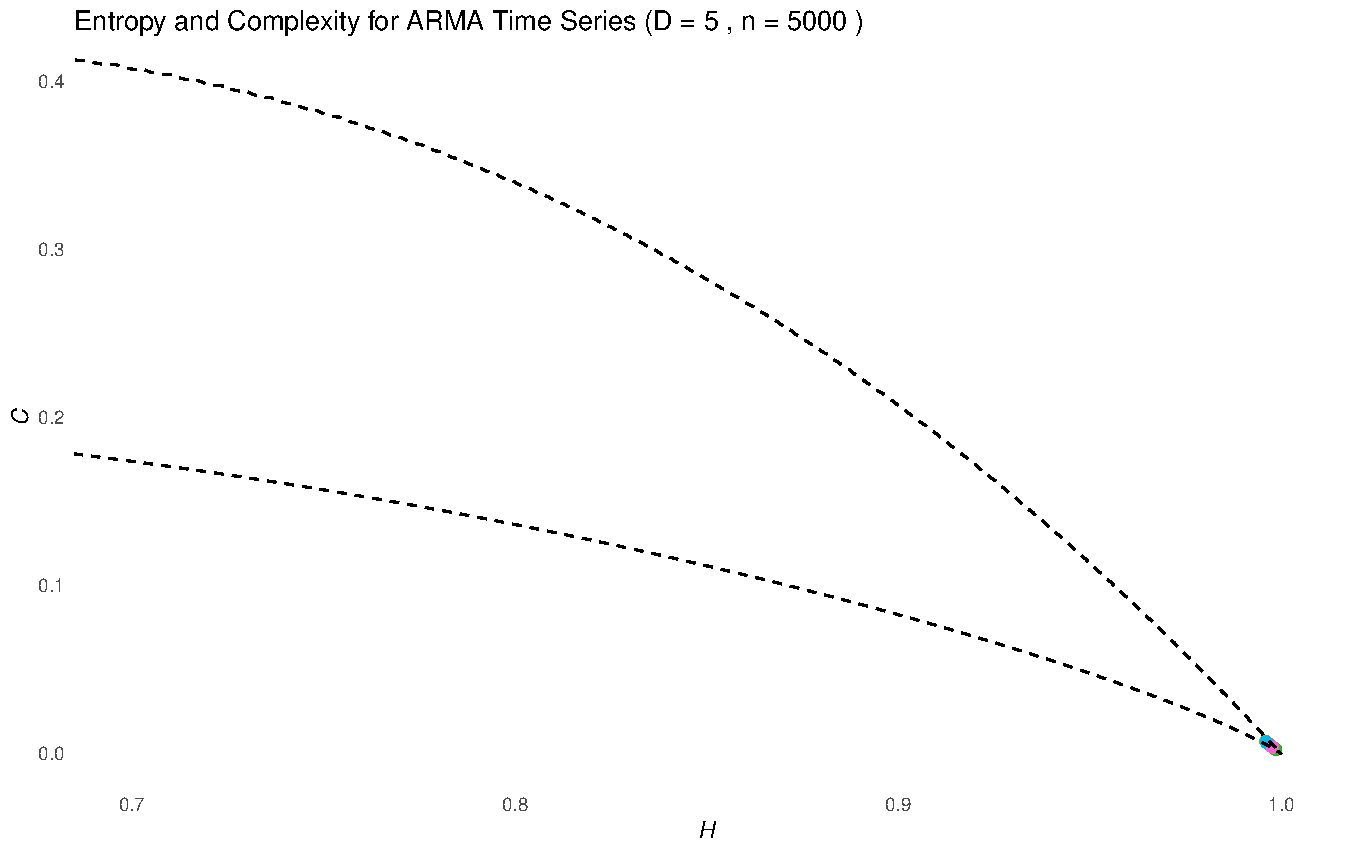
\includegraphics[width=0.8 \textwidth]{HC plane ARMA(22) n5000}
	\caption{$H \times C$ plane for ARMA(2,2) model with parameter condition: Sample size 5000}
	\label{fig:HC ARMA(22) constraint}
\end{figure}	

\begin{figure}[H]
	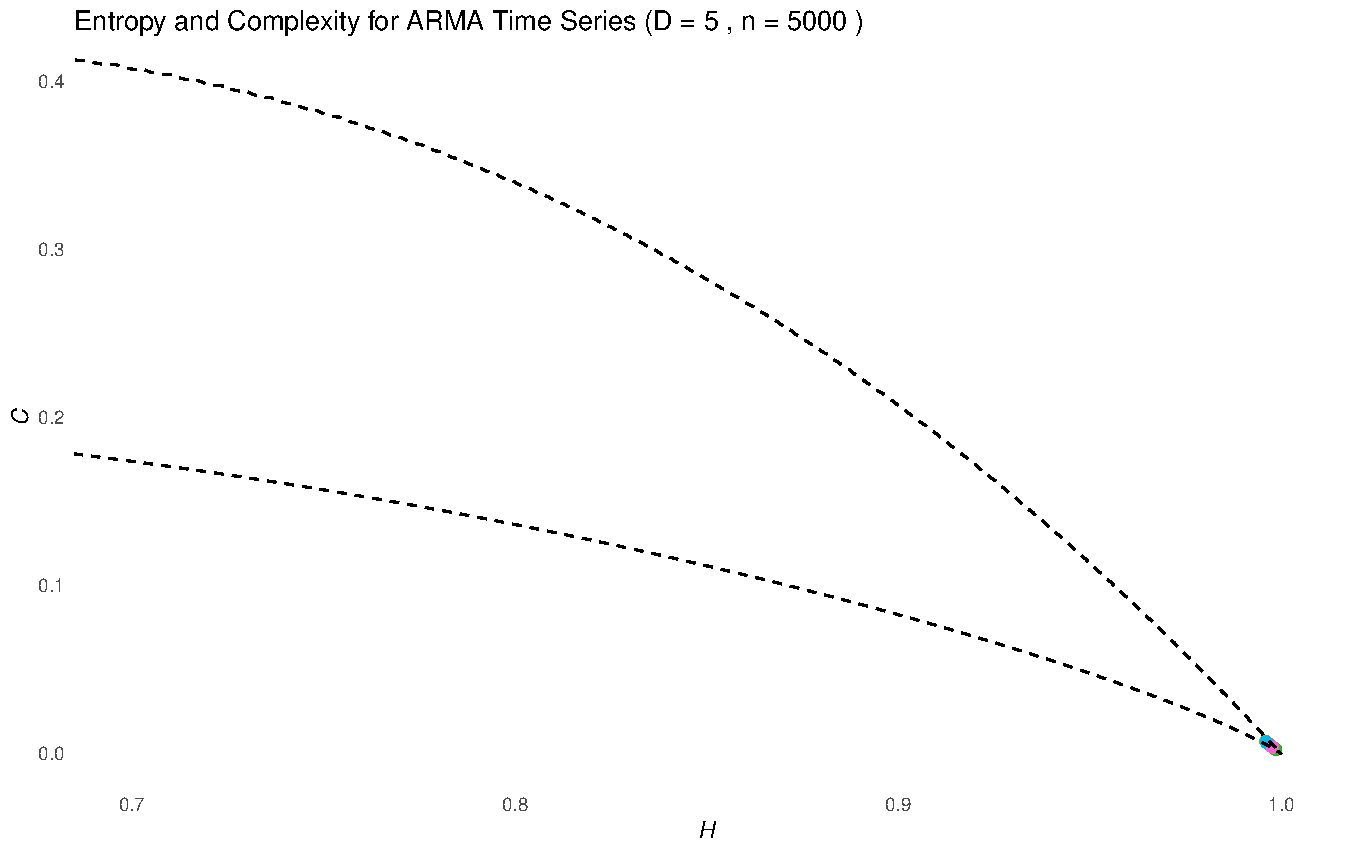
\includegraphics[width=0.8 \textwidth]{HC plane ARMA(22) n5000 without condition}
	\caption{$H \times C$ plane for ARMA(2,2) model without parameter condition: Sample size 5000}
	\label{fig:HC ARMA(22) unconstraint}
\end{figure}

\begin{figure}[H]
	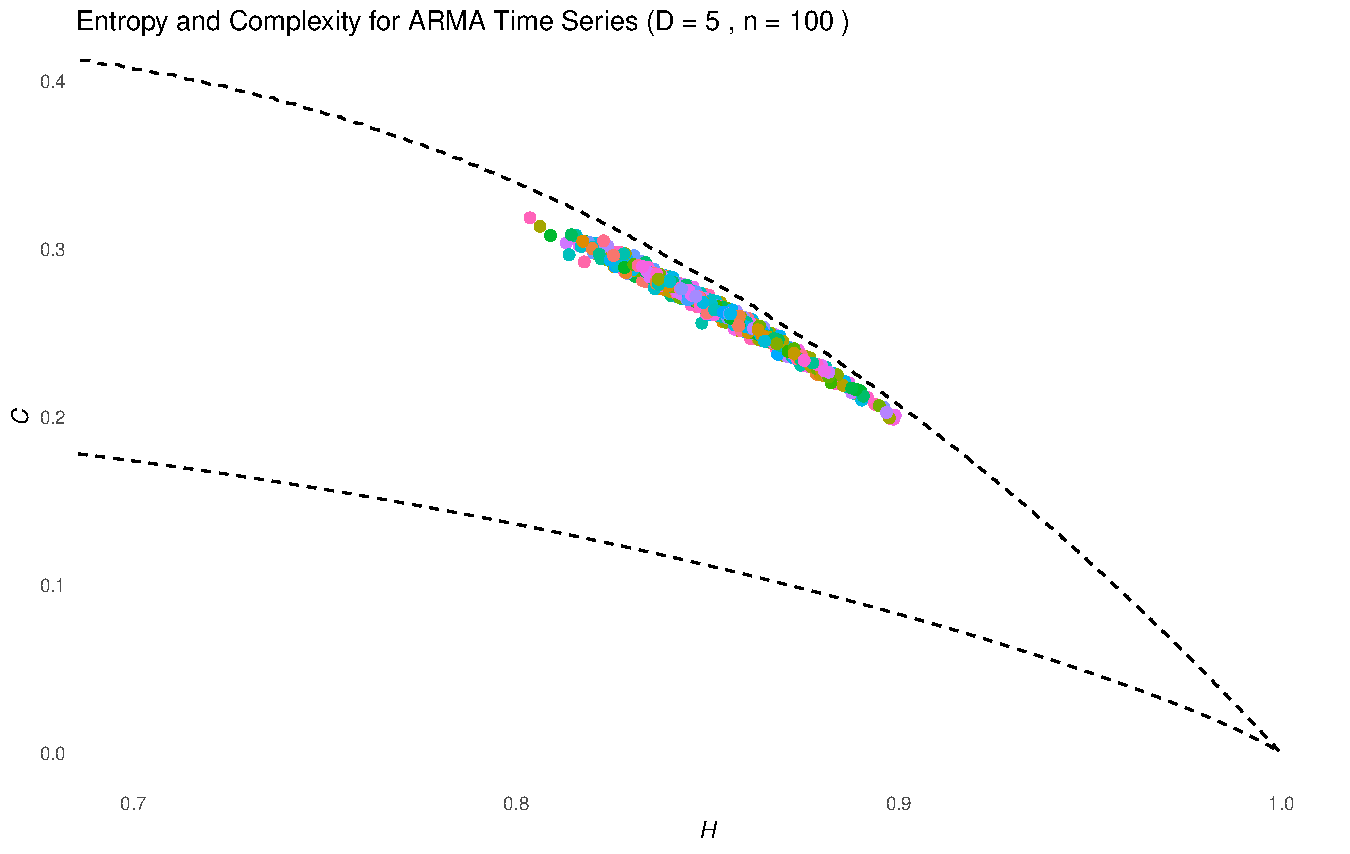
\includegraphics[width=0.8 \textwidth]{HC plane ARMA(22) n100}
	\caption{$H \times C$ plane for ARMA(2,2) model with parameter condition: Sample size 100}
	\label{fig:HC ARMA(22) constraint n100}
\end{figure}

\begin{figure}[H]
	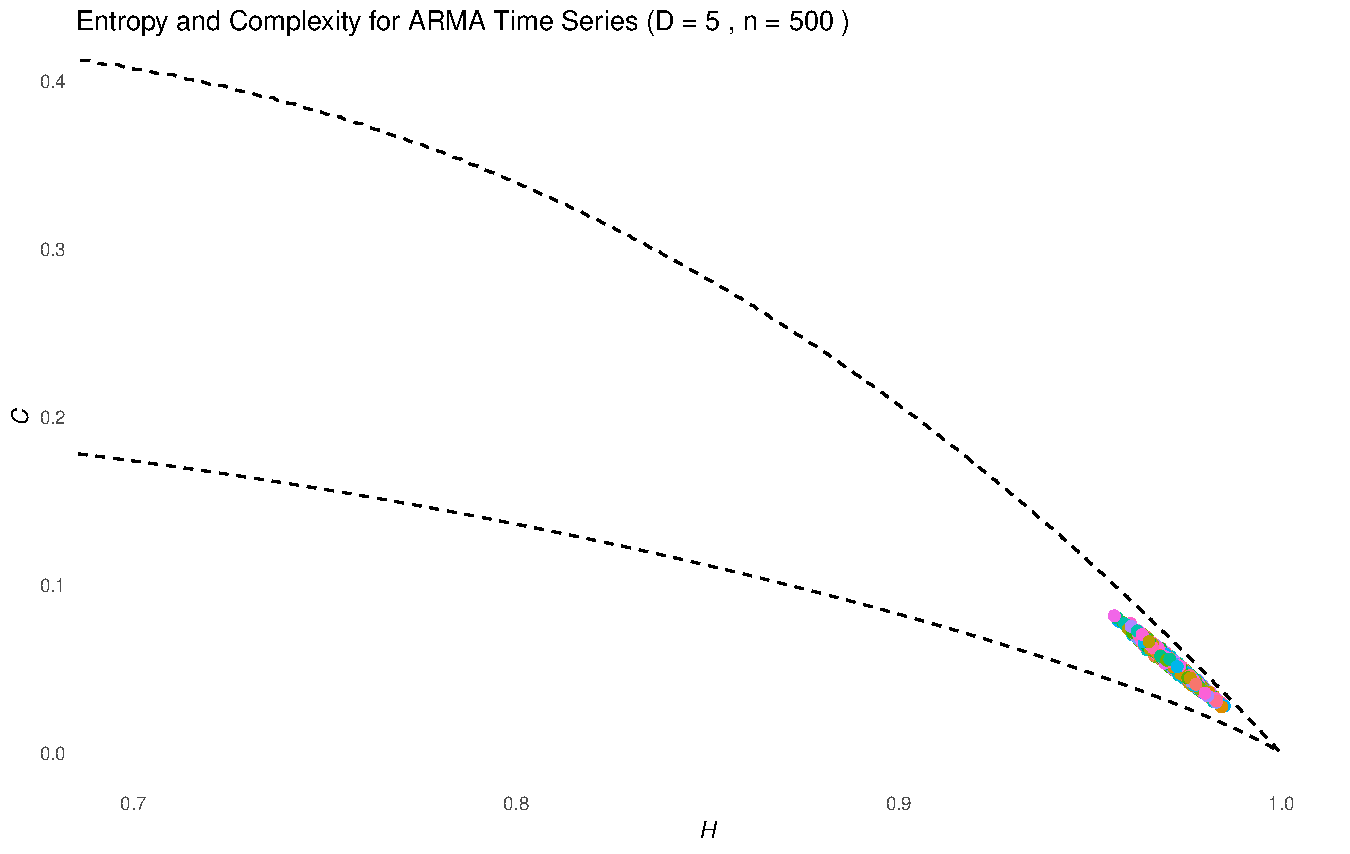
\includegraphics[width=0.8 \textwidth]{HC plane ARMA(22) n500}
	\caption{$H \times C$ plane for ARMA(2,2) model with parameter condition: Sample size 500}
	\label{fig:HC ARMA(22) constraint n500}
\end{figure}			
	
\begin{figure}[H]
	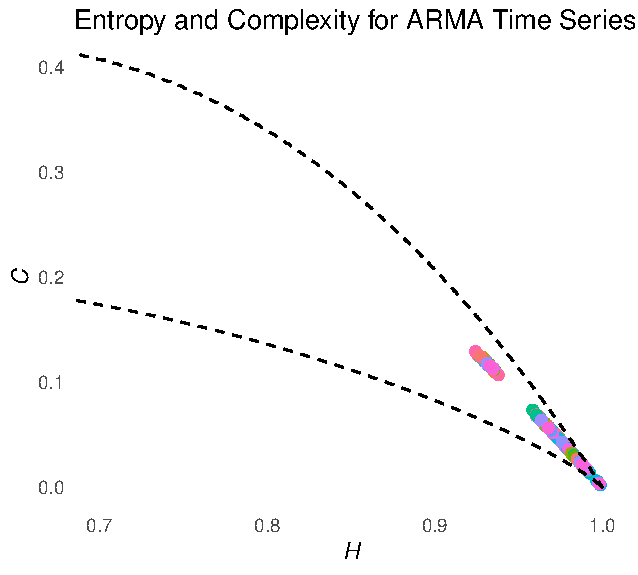
\includegraphics[width=0.8 \textwidth]{HC plane ARMA21 n5000}
	\caption{$H \times C$ plane for ARMA(2,1) model with parameter condition: Sample size 5000}
	\label{fig:HC ARMA(21)}
\end{figure}	

\begin{figure}[H]
	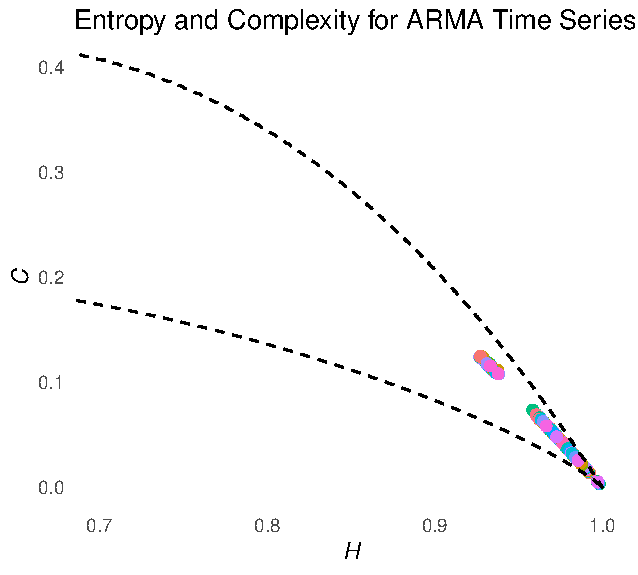
\includegraphics[width=0.8 \textwidth]{HC plane ARMA12 n5000}
	\caption{$H \times C$ plane for ARMA(1,2) model:Sample size 5000}
	\label{fig:HC ARMA(12)}
\end{figure}


\begin{figure}[H]
	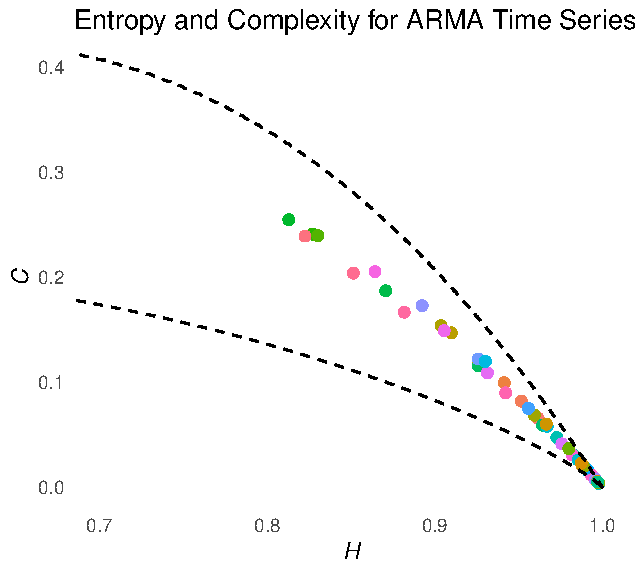
\includegraphics[width=0.8 \textwidth]{HC plane ARMA(11) n5000}
	\caption{$H \times C$ plane for ARMA(1,1) model:Sample size 5000}
	\label{fig:HC ARMA(11)}
\end{figure}

\begin{figure}[H]
	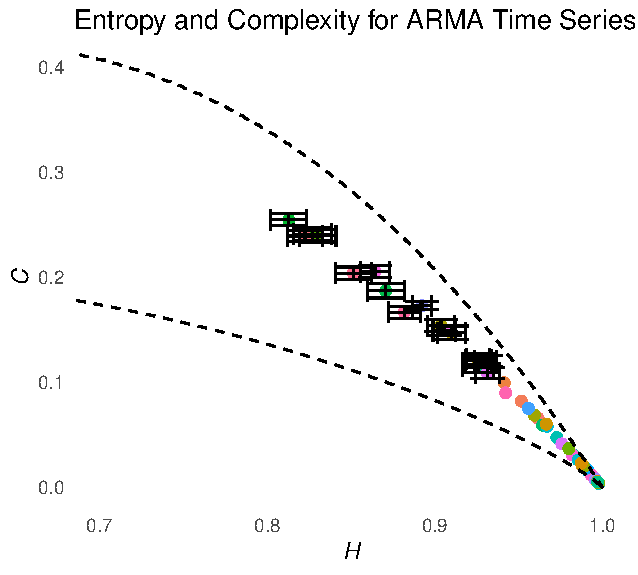
\includegraphics[width=0.8 \textwidth]{HC plane ARMA(11) with CI}
	\caption{$H \times C$ plane for ARMA(1,1) model with Confidence Interval:Sample size 5000}
	\label{fig:HC ARMA(11) CI}
\end{figure}



	
	
%\section{Conclusion and future work}
%These experiments show that using ordinal patterns can help group (cluster) time series data in meaningful ways. First, we kept the model settings the same (AR = 0.6 and MA = 0.3) and changed the sample size (from 500 up to 5000) and the embedding dimension (from 3 to 6) to see how these factors affect measures like entropy and complexity. Then, we focused on one case (embedding dimension 5 and sample size 1000) and changed the ARMA model’s parameters. The results suggest that the way we group time series using ordinal patterns depends on the sample size, the embedding dimension, and the ARMA model’s settings.

%Future Work
%In the future, I plan to include experiments with deterministic chaos (using time series with chaotic behavior) as well as random data. This will help test whether ordinal patterns and complexity-entropy measures can tell the difference between chaos and randomness, and improve clustering results in these new situations.
	
%	\bibliography{../BearingFaultDiagnosis}
	
\end{document}

